% default values
\def\ttau{0.01} % Zeitkonstante tau
%
% Plot Umgebung:
\def\samples{41}
%
\def\xomegaordermin{0}
\def\xomegaordermax{4}
\def\xomegamin{1e\xomegaordermin}
\def\xomegamax{1e\xomegaordermax}
\def\domain{\xomegamin:\xomegamax}
%
\def\yamptiefmin{0.8e-2}    % \ymin needed as macro to draw ycomb with node-text from x-axis to plot
\def\yamptiefmax{2}
%
\def\yamphochmin{0.8e-2}    % \ymin needed as macro to draw ycomb with node-text from x-axis to plot
\def\yamphochmax{2}
%
\def\yphitiefmax{+10}
\def\yphitiefmin{-100}      % \ymin needed as macro to draw ycomb with node-text from x-axis to plot % 1. Ordnung
\def\yphitiefg{-45}
%
\def\yphihochmin{-10}       % \ymin needed as macro to draw ycomb with node-text from x-axis to plot % 1. Ordnung % Alternative: [ycomb, update limits=false] small y value outer bounds but no dynamic node text
\def\yphihochmax{100}
\def\yphihochg{45}
%
%%%%%%%%%%%%%%%%%%%%%%%%%%%%%%%%%%%%%%%%%%%%%%%%%%%%%%%%%%%%%%%%%%%%%%%%%%%%
%
% RC-Tiefpass 1. Ord. Amplitudengang
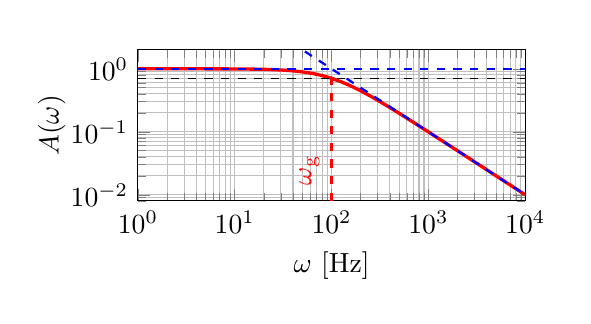
\begin{tikzpicture}[x=1mm,y=1mm] % gilt für tikz-coordinaten außerhalb der axis-environment

    \draw[draw=none] (-14,-12) rectangle (54,22); % Bildrahmen, Koordinatenbezug auf (0,0) des \begin{axis}...\end{axis} pgfplots, für

    \begin{loglogaxis}[
        %title={Amplitudengang RC-Tiefpass 1. Ordnung},
        xlabel={$\omega\ [\mathrm{Hz}]$},
        ylabel={$A(\omega)$},
        ylabel shift = -5pt,
        xmin=\xomegamin, xmax=\xomegamax,
        ymin= 0.8 * 1/(1+(\xomegamax*\ttau)^2)^0.5, % 0.8*0.01 (manual cut off bottom)
        ymax=\yamptiefmax,   % \ymin needed as macro to draw ycomb with node-text from x-axis to plot intersection
        domain=\domain,
        samples=\samples,
        log origin=infty,
        grid=minor,
        width=6.5cm,
        height=3.5cm,
    ]     
        \addplot+[mark=none,very thick,red,]   {1/(1+(x*\ttau)^2)^ 0.5};

        \addplot+[ycomb,dashed,mark=none,thick,red,] coordinates { (1/(\ttau),\yamptiefmin) (1/(\ttau),1/2^0.5)}  node [pos=0.25,sloped,style={yshift=8pt}] {$\omega_{\mathrm{g}}$}; % Grenzfrequenz             
        \addplot+[dashed,mark=none,thick,blue] coordinates { (\xomegamin,1) (\xomegamax,1) };
        \addplot+[dashed,mark=none,thick,blue]   { 1/(x*\ttau) } 
            %coordinate [pos= (\xomegaordermax-0)/(\xomegaordermax-\xomegaordermin) ] (A)
            %coordinate [pos= (\xomegaordermax-1)/(\xomegaordermax-\xomegaordermin) ] (B)
        ;
            %\draw (A) -| (B) node [pos=0.5,anchor=west,yshift=15pt]{$\frac{-20\ dB}{Dek}$}; % slope 20 dB/Dek
        
        \addplot+[dashed,mark=none,black,]  coordinates { (\xomegamin, 1/2^0.5) ( \xomegamax, 1/2^0.5) }   
            node [pos=0,anchor=east,clip=false] {$1/\sqrt{2}$}  % clipped away, otherwise asymptote peaks out above
            %node [pos=0.25,anchor=north] {Durchlassbereich}     % static
            %node [pos=0.75,anchor=north] {Sperrbereich}         % static
        ;        

    \end{loglogaxis}%
\end{tikzpicture}%